%% $Id$
%%
%% Documentation to explain how the scene graph and OpenGL backend is
%% set up and run in FreeWRL.

\documentclass[12pt,letterpaper]{article}

\usepackage{freewrl}
\customheadings

\begin{document}

    The OpenGL libraries do the actual rendering work in the FreeWRL
    browser.
    Setting up the backend is done through FreeWRL's scene model
    \texttt{Scene.pm}.
    The result of the initialization steps described in the next section
    is the scene graph for the VRML input files and the associated backend
    to OpenGL.

    %% better explain the browser class and the event loop!

    \section{FreeWRL Initialization}

	\subsection{Scene Graph}

	The scene graph is a tree constructed by parsing a VRML input file
	starting from the topmost node (how are PROTOs handled?).
	An example of a scene graph corresponding to the following VRML code
	is represented as a tree is shown in Figure~\ref{fig:sg-tree}.

	\begin{verbatim}
	    [pick a VRML example from the FreeWRL tests]
	\end{verbatim}

	\begin{figure}[!ht]
	    \centering
	    \epsfig{file=fig/sg-tree.eps}
	    \caption{}\label{fig:sg-tree}
	\end{figure}

	The browser is responsible for calling the methods to construct the
	scene graph.
	%% lame - needs way more explaination!
	This is done either when a string containing the text of a VRML input
	file is loaded (\texttt{VRML::Browser::load\_string}) or when a world is
	replaced (\texttt{VRML::Browser::replaceWorld}).

	\subsection{Backend}

	During initialization, a series of function calls are made to
	build FreeWRL's backend to OpenGL.
	These function calls are summarized in Figure~\ref{fig:be-setup}.

	\begin{figure}[!ht]
	    \centering
	    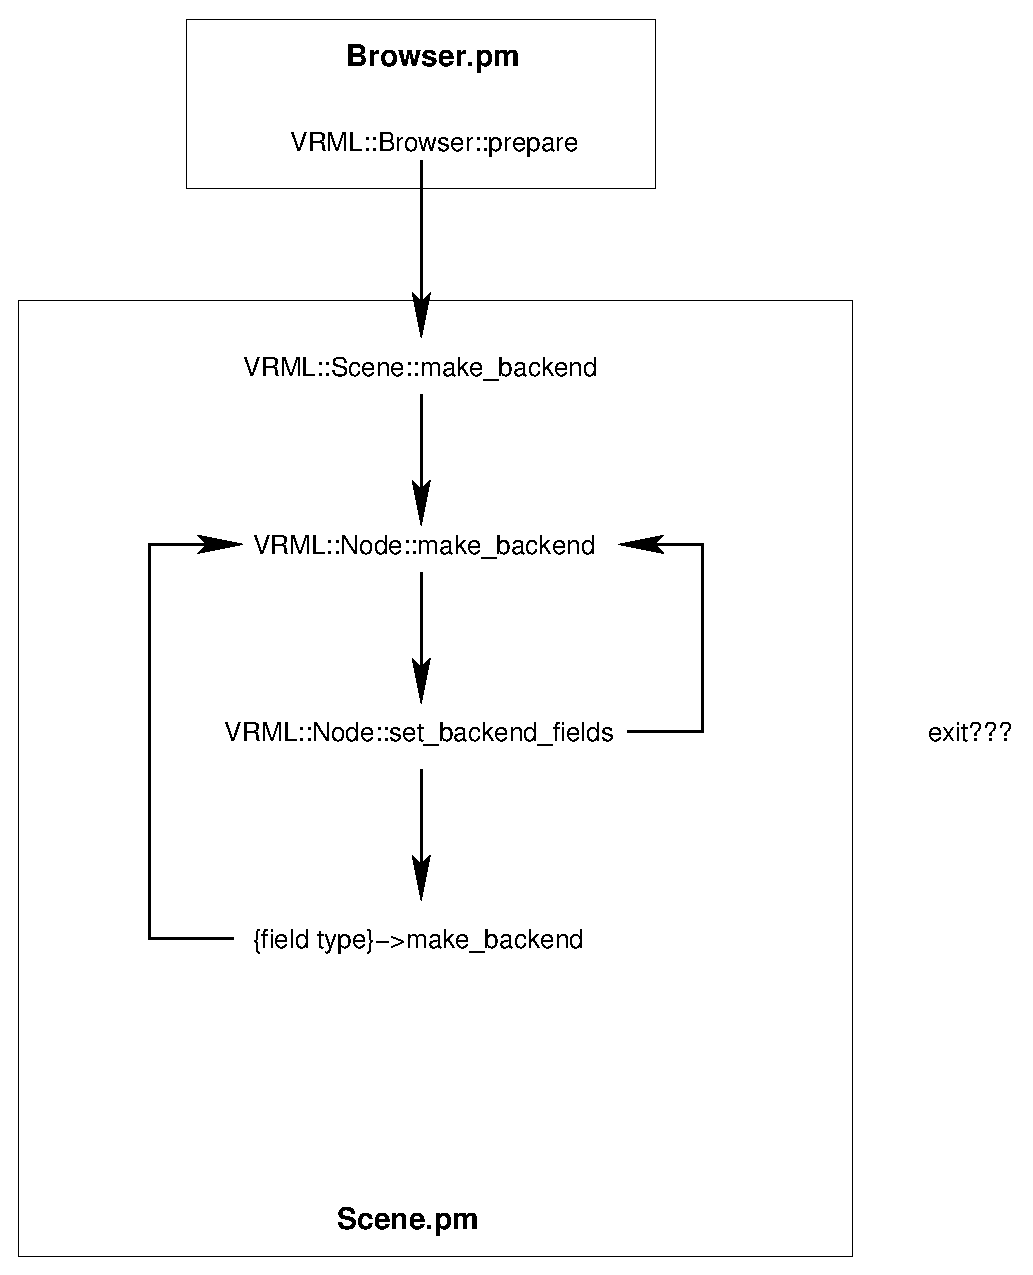
\epsfig{file=fig/be-setup.eps,width=12cm}
	    \caption{Function calls to set up the FreeWRL backend.}\label{fig:be-setup}
	\end{figure}

	The browser contains the backend structure, which is used in the event
	loop to update the scene displayed by FreeWRL.

\end{document}
